\documentclass[12pt,a4paper]{article}

\usepackage[utf8]{inputenc}
\usepackage[T1]{fontenc}
\usepackage[brazil]{babel}
\usepackage{amsmath}
\usepackage{amssymb}
\usepackage{graphicx}
\usepackage{booktabs}
\usepackage{listings}
\usepackage{xcolor}
\usepackage{geometry}
\usepackage{hyperref}

\geometry{margin=2.5cm}

\lstset{
    language=Python,
    basicstyle=\ttfamily\small,
    keywordstyle=\color{blue},
    commentstyle=\color{gray},
    numbers=left,
    numberstyle=\tiny\color{gray},
    frame=single,
    breaklines=true,
    showstringspaces=false
}

\title{Relatório do Sistema do Pêndulo Duplo}
\author{}
\date{}

\begin{document}

\maketitle

\section{Introdução e descrição física do sistema}

O sistema investigado consiste em um pêndulo duplo planar, composto por duas hastes rígidas conectadas em sequência, sujeitas à ação da gravidade. Trata-se de um sistema mecânico clássico de dinâmica não linear, em que o movimento de uma haste influencia diretamente a outra por meio do acoplamento entre os ângulos de rotação.

As grandezas dinâmicas fundamentais do problema são os ângulos de deflexão das hastes em relação à vertical:

\begin{itemize}
    \item $\theta_1$: ângulo da haste 1;
    \item $\theta_2$: ângulo da haste 2.
\end{itemize}

As velocidades angulares associadas são:

\begin{itemize}
    \item $\omega_1 = \dot{\theta}_1$;
    \item $\omega_2 = \dot{\theta}_2$;
\end{itemize}

Assim, o vetor de estado do sistema pode ser escrito como

\begin{equation}
\mathbf{y} = \begin{bmatrix}
\theta_1 \\
\theta_2 \\
\omega_1 \\
\omega_2
\end{bmatrix}.
\end{equation}

No código, essa estrutura é representada por:

\begin{lstlisting}
y = np.array([theta1, theta2, w1, w2])
\end{lstlisting}

e cada componente é acessado por meio da decomposição:

\begin{lstlisting}
theta1, theta2, w1, w2 = y
\end{lstlisting}

Essa correspondência é central para a interpretação física do modelo computacional: cada variável matemática do sistema possui uma analogia direta em termos de coordenadas e velocidades angulares.

\section{Formulação matemática e abstração do sistema}

A dinâmica pode ser escrita como um sistema de equações diferenciais ordinárias de primeira ordem:

\begin{equation}
\frac{d}{dt}
\begin{bmatrix}
\theta_1 \\
\theta_2 \\
\omega_1 \\
\omega_2
\end{bmatrix}
=
\begin{bmatrix}
\omega_1 \\
\omega_2 \\
\alpha_1 \\
\alpha_2
\end{bmatrix},
\end{equation}

em que $\alpha_1$ e $\alpha_2$ representam as acelerações angulares das hastes.

Essa representação é equivalente à implementação:

\begin{lstlisting}
def derivadas(y, g=9.8, l=1.0):
    a1, a2 = aceleracoes(y, g=9.8, l=1.0)
    return np.array([y[2], y[3], a1, a2])
\end{lstlisting}

A equivalência entre as variáveis é:

\begin{itemize}
    \item \texttt{y[0] = theta1 = $\theta_1$};
    \item \texttt{y[1] = theta2 = $\theta_2$};
    \item \texttt{y[2] = w1 = $\omega_1$};
    \item \texttt{y[3] = w2 = $\omega_2$};
    \item a saída do vetor é \texttt{[$\omega_1$, $\omega_2$, $\alpha_1$, $\alpha_2$]}.
\end{itemize}

Essa reformulação transforma um problema de segunda ordem em um sistema de primeira ordem compatível com métodos como o Runge--Kutta.

\section{Acelerações angulares e acoplamento dinâmico}

A dinâmica depende da diferença angular entre as duas hastes:

\begin{equation}
\Delta = \theta_1 - \theta_2.
\end{equation}

No código, essa quantidade é calculada por:

\begin{lstlisting}
delta = theta1 - theta2
\end{lstlisting}

A variável $\Delta$ é central para o acoplamento entre as partes do sistema. Ela incorpora a não linearidade, pois a resposta de cada haste depende da configuração instantânea da outra.

O denominador utilizado nas acelerações é

\begin{equation}
D = 16 - 9\cos^2(\Delta).
\end{equation}

Na implementação:

\begin{lstlisting}
den = 16 - 9 * np.cos(delta) ** 2
\end{lstlisting}

As acelerações angulares são:

\begin{align}
\alpha_1 &= -\frac{3\left(2\omega_2^2\sin\Delta
+3\cos\Delta\,\omega_1^2\sin\Delta
+6\frac{g}{l}\sin\theta_1
-3\cos\Delta\frac{g}{l}\sin\theta_2\right)}{D},\\
\alpha_2 &= \frac{3\left(8\omega_1^2\sin\Delta
+3\cos\Delta\,\omega_2^2\sin\Delta
-8\frac{g}{l}\sin\theta_2
+9\cos\Delta\frac{g}{l}\sin\theta_1\right)}{D}.
\end{align}

No código:

\begin{lstlisting}
a1 = -3*(2*w2**2*np.sin(delta) + 3*np.cos(delta)*w1**2*np.sin(delta)
         + 6*(g/l)*np.sin(theta1) - 3*np.cos(delta)*(g/l)*np.sin(theta2)) / den
a2 =  3*(8*w1**2*np.sin(delta) + 3*np.cos(delta)*w2**2*np.sin(delta)
         - 8*(g/l)*np.sin(theta2) + 9*np.cos(delta)*(g/l)*np.sin(theta1)) / den
\end{lstlisting}

A correspondência entre as variáveis matemáticas e computacionais é:

\begin{itemize}
    \item \texttt{theta1} $\leftrightarrow \theta_1$;
    \item \texttt{theta2} $\leftrightarrow \theta_2$;
    \item \texttt{w1} $\leftrightarrow \omega_1$;
    \item \texttt{w2} $\leftrightarrow \omega_2$;
    \item \texttt{delta} $\leftrightarrow \Delta$;
    \item \texttt{den} $\leftrightarrow D$;
    \item \texttt{g} $\leftrightarrow g$;
    \item \texttt{l} $\leftrightarrow l$;
    \item \texttt{a1} $\leftrightarrow \alpha_1$;
    \item \texttt{a2} $\leftrightarrow \alpha_2$.
\end{itemize}

Essas relações demonstram como o modelo físico é traduzido para a linguagem computacional adotada pelo algoritmo.

\section{Energia mecânica do sistema}

A energia total do pêndulo duplo é composta pela energia cinética e pela energia potencial gravitacional.

\subsection{Energia cinética}

\begin{equation}
T = \frac{m l^2}{6}\left(4\omega_1^2+\omega_2^2
+3\omega_1\omega_2\cos(\theta_1-\theta_2)\right).
\end{equation}

\subsection{Energia potencial}

\begin{equation}
U = -\frac{1}{2}mgl\left(3\cos\theta_1+\cos\theta_2\right).
\end{equation}

\subsection{Energia total}

\begin{equation}
E = T + U.
\end{equation}

A expressão é implementada por:

\begin{lstlisting}
def energia(y, m=1.0, g=9.8, l=1.0):
    th1, th2, w1, w2 = y
    T = m*l**2/6 * (4*w1**2 + w2**2
                     + 3*w1*w2*np.cos(th1-th2))
    U = -0.5*m*g*l * (3*np.cos(th1) + np.cos(th2))
    return T + U
\end{lstlisting}

A análise da energia oferece uma validação qualitativa do modelo: em um sistema conservativo ideal, a energia total deve variar pouco ao longo do tempo. Pequenas oscilações são esperadas pela discretização numérica.

\section{Método numérico: Runge--Kutta de quarta ordem}

A simulação aproxima a solução de problemas de valor inicial:

\begin{equation}
\frac{d\mathbf{y}}{dt}=\mathbf{f}(t,\mathbf{y}).
\end{equation}

A atualização pelo método RK4 é

\begin{equation}
\mathbf{y}_{n+1}=\mathbf{y}_n+
\frac{h}{6}(k_1+2k_2+2k_3+k_4),
\end{equation}

onde

\begin{align}
k_1 &= f(t_n,\mathbf{y}_n),\\
k_2 &= f\left(t_n+\frac{h}{2},\mathbf{y}_n+\frac{h}{2}k_1\right),\\
k_3 &= f\left(t_n+\frac{h}{2},\mathbf{y}_n+\frac{h}{2}k_2\right),\\
k_4 &= f(t_n+h,\mathbf{y}_n+hk_3).
\end{align}

No código:

\begin{lstlisting}
def rk4(fun, tempos, y0):
    y = [y0]
    dt = tempos[1] - tempos[0]

    for t in tempos[:-1]:
        k1 = fun(t, y[-1])
        k2 = fun(t + dt/2, y[-1] + k1*dt/2)
        k3 = fun(t + dt/2, y[-1] + k2*dt/2)
        k4 = fun(t + dt, y[-1] + dt*k3)
        y.append(y[-1] + dt/6
                 * (k1 + 2*k2 + 2*k3 + k4))

    return np.array(y)
\end{lstlisting}

O passo temporal é

\begin{equation}
h=t_{n+1}-t_n.
\end{equation}

Esse método é adequado para sistemas dinâmicos não lineares, pois oferece maior precisão e estabilidade que esquemas mais simples.

\section{Dinâmica do movimento do pêndulo duplo}

O movimento resulta da ação simultânea da gravidade, da inércia das duas hastes e do vínculo que une suas extremidades. Cada haste possui movimento angular próprio, descrito pelos pares $(\theta_1,\omega_1)$ e $(\theta_2,\omega_2)$. Esses pares não evoluem independentemente: a posição e a velocidade de uma haste modificam a aceleração da outra.

A não linearidade aparece nas funções trigonométricas e no acoplamento dos termos quadráticos das velocidades. Dependendo das condições iniciais, o sistema pode apresentar oscilações, inversões rápidas e movimento irregular.

Matematicamente, a dinâmica é integrada pelo sistema

\begin{equation}
\dot{\theta}_1=\omega_1,
\qquad
\dot{\theta}_2=\omega_2,
\qquad
\dot{\omega}_1=\alpha_1,
\qquad
\dot{\omega}_2=\alpha_2.
\end{equation}

Sem atrito ou dissipação, a energia mecânica se conserva. Durante a descida das hastes, a energia potencial é convertida em energia cinética. Durante a subida, ocorre o processo inverso.

\section{Condição inicial e interpretação do movimento}

A simulação original parte da condição:

\begin{lstlisting}
y0 = np.array([np.pi/2, np.pi/2, 0.0, 0.0])
\end{lstlisting}

isto é,

\begin{equation}
\theta_1(0)=\frac{\pi}{2},
\quad
\theta_2(0)=\frac{\pi}{2},
\quad
\omega_1(0)=0,
\quad
\omega_2(0)=0.
\end{equation}

Esse estado corresponde a duas hastes inicialmente horizontais e em repouso. Sob a ação da gravidade, o sistema evolui para movimentos amplos e não lineares.

\section{Trajetória da extremidade da haste 2}

As coordenadas cartesianas da extremidade são

\begin{align}
x_2 &= l\sin\theta_1+l\sin\theta_2,\\
y_2 &= -l\cos\theta_1-l\cos\theta_2.
\end{align}

No programa:

\begin{lstlisting}
x2 = l*np.sin(Y[:, 0]) + l*np.sin(Y[:, 1])
y2 = -l*np.cos(Y[:, 0]) - l*np.cos(Y[:, 1])
\end{lstlisting}

O par $(x_2,y_2)$ representa a posição espacial da extremidade da segunda haste ao longo do tempo. A trajetória observada reflete a evolução conjunta dos ângulos e a dinâmica do acoplamento entre as hastes.

\section{Análise da energia ao longo da simulação}

A evolução da energia é calculada por:

\begin{lstlisting}
Es = np.array([energia(y) for y in Y])
print("deriva máxima da energia:",
      np.max(np.abs(Es-Es[0])))
\end{lstlisting}

A diferença em relação ao estado inicial é

\begin{equation}
\Delta E(t)=E(t)-E(0).
\end{equation}

Em um modelo conservativo ideal, essa diferença deve permanecer pequena. Variações próximas de zero indicam consistência da formulação e do método numérico.

\section{Interpretação abstrata do sistema dinâmico}

O pêndulo duplo é um sistema de dimensão quatro:

\begin{equation}
\mathbf{y}=\left(\theta_1,\theta_2,\omega_1,\omega_2\right).
\end{equation}

Portanto, o espaço de estados é quatro-dimensional. A dinâmica é não linear e o acoplamento entre as hastes pode fazer pequenas alterações nas condições iniciais produzirem trajetórias muito diferentes. Essa propriedade é associada ao comportamento caótico.

\section{Comparação das condições iniciais e comportamento caótico}

Foram comparadas duas condições iniciais. Na condição original, ambas as hastes começam na horizontal e em repouso:

\begin{equation}
\theta_1(0)=\frac{\pi}{2},\quad
\theta_2(0)=\frac{\pi}{2},\quad
\omega_1(0)=0,\quad
\omega_2(0)=0.
\end{equation}

Na condição perturbada, as posições são mantidas, mas são atribuídas velocidades angulares iniciais:

\begin{equation}
\theta_1(0)=\frac{\pi}{2},\quad
\theta_2(0)=\frac{\pi}{2},\quad
\omega_1(0)=0{,}25,\quad
\omega_2(0)=0{,}25.
\end{equation}

A perturbação adiciona energia cinética e modifica o modo como as hastes trocam energia potencial e cinética. As trajetórias deixam de ser curvas simples e periódicas e passam a apresentar mudanças contínuas de direção.

\begin{figure}[htbp]
    \centering
    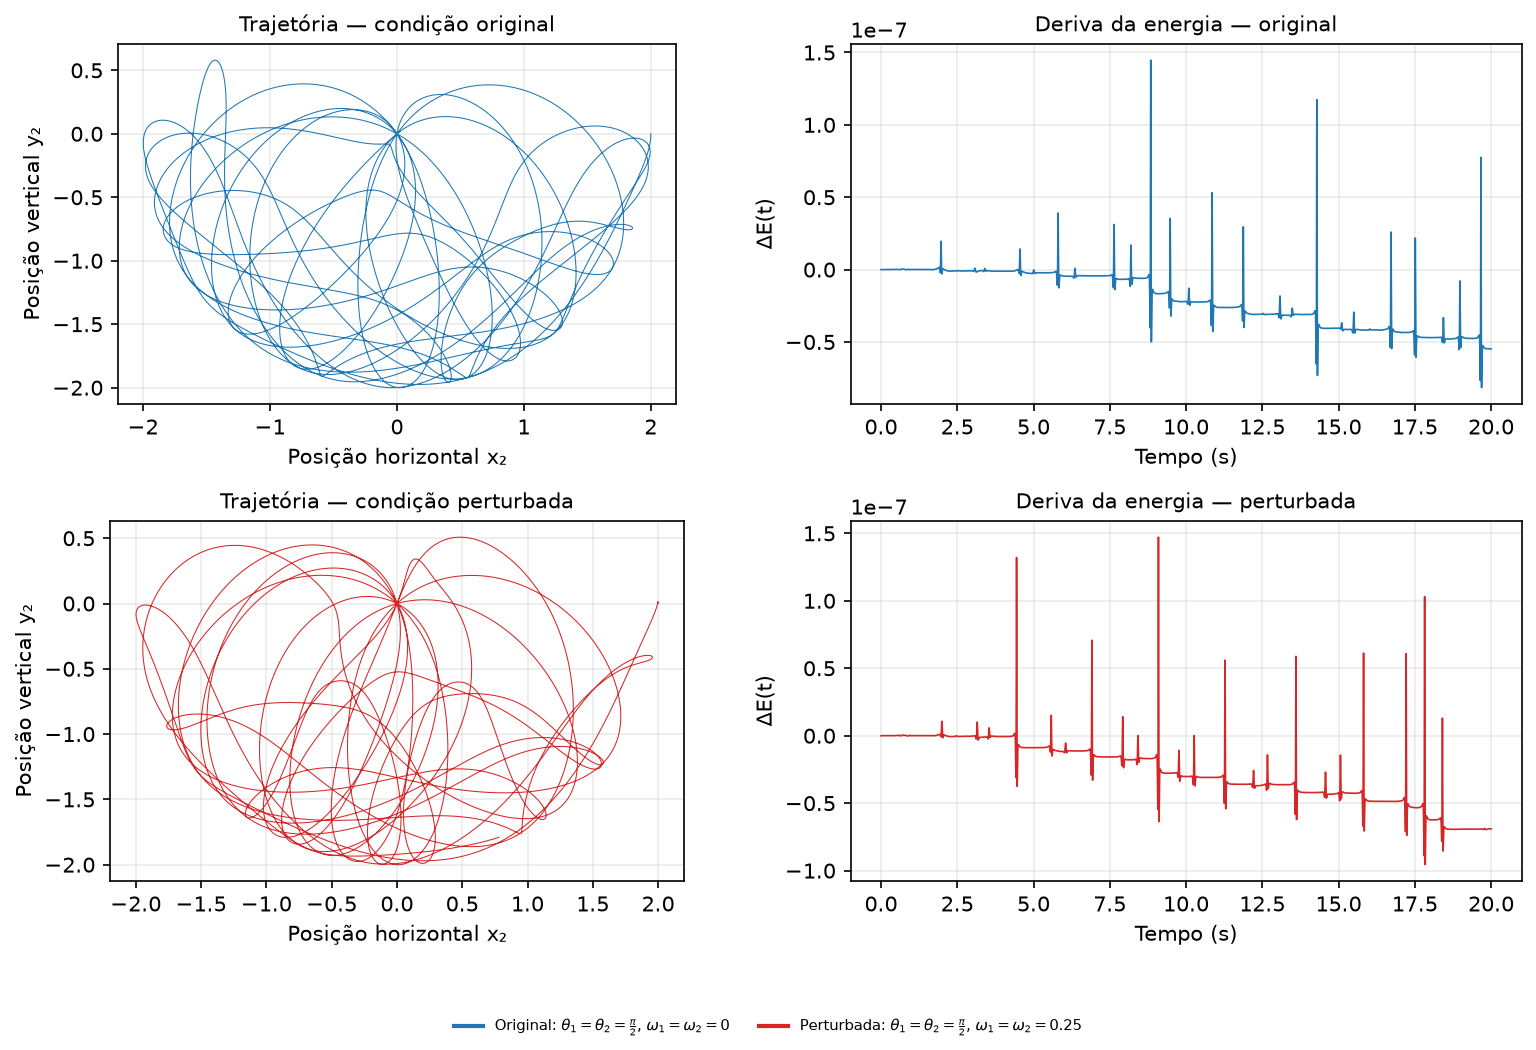
\includegraphics[width=0.95\textwidth]{pendulo_duplo_comparacao.png}
    \caption{Comparação das trajetórias da extremidade e da deriva da energia para as condições original e perturbada.}
    \label{fig:comparacao_pendulo}
\end{figure}

Os gráficos superiores da Figura~\ref{fig:comparacao_pendulo} correspondem à condição original e os inferiores à condição perturbada. As curvas azuis representam o caso sem velocidades iniciais, enquanto as curvas vermelhas representam o caso perturbado.

Essa diferença é uma manifestação da sensibilidade às condições iniciais. Como o sistema é não linear e possui acoplamento entre $\theta_1$ e $\theta_2$, uma variação no estado inicial pode crescer ao longo do tempo. Assim, trajetórias inicialmente próximas podem tornar-se progressivamente distintas.

Os gráficos da direita apresentam $\Delta E(t)=E(t)-E(0)$. Pequenas oscilações próximas de zero mostram que o método RK4 conserva razoavelmente a energia. Dessa forma, as diferenças observadas nas trajetórias estão associadas principalmente às condições iniciais e à não linearidade do modelo, e não à perda artificial de energia.

A condição perturbada não possui necessariamente movimento periódico previsível. O acoplamento entre as hastes e os termos trigonométricos das equações produzem forças que alteram continuamente a direção e a velocidade das massas. Esse processo gera trajetórias irregulares e mudanças súbitas no sentido de giro.

O comportamento observado é característico de caos determinístico: a evolução é completamente definida pelas equações e pela condição inicial, mas a previsão prática torna-se difícil para tempos longos. Uma pequena variação em qualquer componente de $\mathbf{y}$ pode ser amplificada pela dinâmica não linear.

\section{Variáveis utilizadas nas condições comparadas}

No notebook, as duas condições simuladas são armazenadas nos vetores de estado

\begin{equation}
\mathbf{y}_0
=
\begin{bmatrix}
\theta_1(0)\\
\theta_2(0)\\
\omega_1(0)\\
\omega_2(0)
\end{bmatrix}
=
\begin{bmatrix}
\pi/2\\
\pi/2\\
0\\
0
\end{bmatrix}
\end{equation}

para a condição original e

\begin{equation}
\mathbf{y}_1
=
\begin{bmatrix}
\theta_1(0)\\
\theta_2(0)\\
\omega_1(0)\\
\omega_2(0)
\end{bmatrix}
=
\begin{bmatrix}
\pi/2\\
\pi/2\\
0{,}25\\
0{,}25
\end{bmatrix}
\end{equation}

para a condição perturbada.

As respectivas implementações são:

\begin{lstlisting}
y0 = np.array([np.pi/2, np.pi/2, 0.0, 0.0])
Y = rk4(fun, tempos, y0)

y1 = np.array([np.pi/2, np.pi/2, 0.25, 0.25])
Y1 = rk4(fun, tempos, y1)
\end{lstlisting}

Assim, $Y$ contém a evolução da condição original e $Y1$ contém a evolução da condição perturbada. A energia mecânica associada a cada trajetória é armazenada em $Es$ e $Es1$, respectivamente:

\begin{lstlisting}
Es = np.array([energia(y) for y in Y])
Es1 = np.array([energia(y) for y in Y1])
\end{lstlisting}

As coordenadas da extremidade da segunda haste são obtidas a partir de cada solução por

\begin{lstlisting}
x2 = l*np.sin(Y[:, 0]) + l*np.sin(Y[:, 1])
y2 = -l*np.cos(Y[:, 0]) - l*np.cos(Y[:, 1])

x = l*np.sin(Y1[:, 0]) + l*np.sin(Y1[:, 1])
y = -l*np.cos(Y1[:, 0]) - l*np.cos(Y1[:, 1])
\end{lstlisting}

Portanto, $(x_2,y_2)$ representa a trajetória da condição original, enquanto $(x,y)$ representa a trajetória da condição perturbada. A presença de velocidades iniciais nos componentes $\omega_1$ e $\omega_2$ modifica diretamente as acelerações e a redistribuição de energia entre as hastes.

\section{Conclusão}

O modelo matemático e a implementação computacional do pêndulo duplo são coerentes entre si. As principais grandezas envolvidas são:

\begin{itemize}
    \item $\theta_1$ e $\theta_2$: ângulos das hastes;
    \item $\omega_1$ e $\omega_2$: velocidades angulares;
    \item $g$: aceleração gravitacional;
    \item $l$: comprimento das hastes;
    \item $m$: massa;
    \item $\Delta=\theta_1-\theta_2$: diferença angular de acoplamento.
\end{itemize}

Assim, o programa traduz em linguagem computacional a estrutura física e matemática do sistema. A integração numérica, a energia e a trajetória geométrica constituem ferramentas complementares para compreender a dinâmica do pêndulo duplo e avaliar a validade da representação adotada.

\subsection{Origem matemática da não linearidade e do caos}

Define-se o vetor de estado

\begin{equation}
\mathbf{y}=\begin{bmatrix}
\theta_1\\
\theta_2\\
\omega_1\\
\omega_2
\end{bmatrix}
\end{equation}

e o campo vetorial

\begin{equation}
\dot{\mathbf{y}}=\mathbf{F}(\mathbf{y})=
\begin{bmatrix}
\omega_1\\
\omega_2\\
\alpha_1(\theta_1,\theta_2,\omega_1,\omega_2)\\
\alpha_2(\theta_1,\theta_2,\omega_1,\omega_2)
\end{bmatrix}.
\end{equation}

Como o sistema não possui dependência explícita do tempo, ele é autônomo. Sua não linearidade decorre principalmente de quatro fatores:

\begin{enumerate}
    \item os termos gravitacionais dependem de $\sin\theta_1$ e $\sin\theta_2$;
    \item o acoplamento depende de $\cos(\theta_1-\theta_2)$;
    \item aparecem velocidades angulares ao quadrado;
    \item as acelerações são divididas por
    $D=16-9\cos^2(\theta_1-\theta_2)$.
\end{enumerate}

Assim, não é possível resolver o sistema por superposição de modos independentes. Para pequenas oscilações,

\begin{equation}
\sin\theta_i\approx\theta_i,
\qquad
\cos(\theta_1-\theta_2)\approx1,
\end{equation}

mas essa aproximação deixa de representar corretamente movimentos largos.

A variação infinitesimal do estado é descrita pelo jacobiano

\begin{equation}
J(\mathbf{y})=\frac{\partial\mathbf{F}}{\partial\mathbf{y}}.
\end{equation}

Para uma perturbação $\delta\mathbf{y}$ ao redor de uma trajetória $\mathbf{y}(t)$,

\begin{equation}
\frac{d}{dt}(\delta\mathbf{y})
\approx J(\mathbf{y}(t))\,\delta\mathbf{y}.
\end{equation}

Como $J$ depende das posições e velocidades instantâneas, a separação entre duas soluções não permanece constante. Em regiões onde a dinâmica apresenta instabilidade,

\begin{equation}
\|\delta\mathbf{y}(t)\|
\approx
\|\delta\mathbf{y}(0)\|e^{\lambda t},
\end{equation}

onde $\lambda$ pode ser interpretado como um expoente característico positivo ou um expoente de Lyapunov médio. Esse crescimento não torna o movimento aleatório: a trajetória continua determinada pelas equações. Porém, torna difícil prever tempos longos sem conhecer com extrema precisão a condição inicial.

Os termos com $\omega_1^2$ e $\omega_2^2$ representam efeitos inerciais dependentes da própria velocidade. Os termos trigonométricos alteram a geometria das forças gravitacionais. Além disso, $D$ modifica a intensidade do acoplamento conforme a diferença $\theta_1-\theta_2$ varia. Quando uma haste atravessa uma configuração crítica, sua aceleração pode redistribuir rapidamente energia para a outra haste.

No sistema ideal, sem atrito,

\begin{equation}
E=T+U,
\end{equation}

sendo

\begin{align}
T&=\frac{ml^2}{6}\left(4\omega_1^2+\omega_2^2
+3\omega_1\omega_2\cos(\theta_1-\theta_2)\right),\\
U&=-\frac12mgl\left(3\cos\theta_1+\cos\theta_2\right).
\end{align}

Como o sistema é conservativo,

\begin{equation}
\frac{dE}{dt}=0.
\end{equation}

Portanto, uma trajetória não ocupa arbitrariamente todo o espaço de estados: ela permanece sobre uma superfície definida pela energia inicial. Embora exista essa restrição, ela não impede movimento caótico, pois o fluxo pode ocupar regiões irregulares sem repetir exatamente sua trajetória.

Para duas condições próximas,

\begin{equation}
\mathbf{y}_2(0)=\mathbf{y}_1(0)+\delta\mathbf{y}_0,
\end{equation}

a separação entre elas pode ser medida por

\begin{equation}
\varepsilon(t)=\left\|\mathbf{y}_2(t)-\mathbf{y}_1(t)\right\|.
\end{equation}

Na comparação deste relatório, a condição perturbada utiliza

\begin{equation}
\omega_1(0)=0{,}25,
\qquad
\omega_2(0)=0{,}25.
\end{equation}

Essa alteração introduz energia cinética adicional e modifica a dinâmica ao longo de todo o intervalo. Mesmo uma perturbação limitada pode ser ampliada pelo acoplamento não linear.

Assim, o caos no pêndulo duplo não é produzido por forças aleatórias ou pelo método RK4. Ele resulta de um sistema determinístico, não linear, acoplado e sensível às condições iniciais. O método numérico aproxima cada trajetória; em intervalos longos, diferenças diminutas na condição inicial ou no erro acumulado podem direcionar a solução por configurações muito distintas.

\end{document}
